% !TeX spellcheck = en_GB
\documentclass[12pt]{beamer}

% ---------- Beamer setup ----------
\usetheme{default}
\setbeamertemplate{navigation symbols}{}
\setbeamertemplate{footline}{\hfill \scriptsize \insertframenumber \hspace{2ex} \vskip8pt}
\usefonttheme{professionalfonts}

% ---------- Encoding & fonts ----------
\usepackage[T1]{fontenc}
\usepackage[utf8]{inputenc}
\usepackage{lmodern}

% ---------- Graphics & colors ----------
\usepackage{graphicx}
\graphicspath{{assets/}}
\usepackage{xcolor}
\definecolor{darkblue}{RGB}{0,0,139}

% ---------- TikZ / PGFPlots ----------
\usepackage{tikz}
\usetikzlibrary{arrows.meta,positioning,calc,matrix}
\usepackage{pgfplots}
\pgfplotsset{compat=1.18}

% ---------- Math & algos ----------
\usepackage{amsmath, bm}
\usepackage{algorithm}
\usepackage{algpseudocode}

% ---------- Tables ----------
\usepackage{booktabs}

% ---------- Links & QR ----------
\usepackage{hyperref}
\usepackage{qrcode}
\hypersetup{
	colorlinks=true,
	linkcolor=darkblue,
	urlcolor=darkblue,
	pdftitle={Data • Model • Loss (Open Resource)},
	pdfpagemode=UseNone
}

% ---------- Glossaries ----------
% Prefer glossaries-extra to avoid makeglossaries step


% define the extra glossary type *before* loading entries


\usepackage[abbreviations]{glossaries-extra}
\makenoidxglossaries
\input{../assets/ml_macros.tex} % keep in repo
\newglossary[mlg]{math}{mls}{mln}{Mathematical Terms}
\loadglsentries{../ADictML_Glossary_English.tex} % relative path in repo

% ---------- Title ----------
\title{Data • Model • Loss}
\subtitle{An open resource from the Aalto Dictionary of ML}
\author{Alexander Jung}
\date{\today}


\begin{document}
	\begin{frame}
		\titlepage
		\vspace{3mm}
		\footnotesize Licensed under CC BY 4.0 \quad
		\qrcode{https://github.com/AaltoDictionaryofML/AaltoDictionaryofML.github.io}
	\end{frame}
	
	
	\begin{frame}{At a glance — goals}
		\begin{itemize}
			\item Understand the three components of \gls{ml}: \gls{data}, \gls{model}, \gls{loss}.
			\item Identify \glspl{feature} vs \glspl{label} in common modalities (image, audio).
			\item Explain how a \gls{hypothesis} maps \(\featurespace \to \labelspace\).
			\item Compare common \glspl{lossfunc} and when to use them.
		\end{itemize}
	\end{frame}
	

	
	\begin{frame}{\Gls{datapoint} = An Image $\datapoint$}
			% Image as a datapoint
			\begin{minipage}[t]{0.4\textwidth}
				\centering
				\includegraphics[width=\textwidth]{/Users/junga1/AaltoDictionaryofML.github.io/assets/CowsAustria.jpg}
				\vspace{1mm}
			\end{minipage}

				\Glspl{feature}:
				\begin{itemize}
					\item $x_{1}, \,\ldots, \,x_{\nrfeatures}$: Colour intensities of all image pixels.
					\item $x_{\nrfeatures+1}$: Time-stamp of the image capture.
					\item $x_{\nrfeatures+2}$: Spatial location of the image capture.
				\end{itemize}
				\Glspl{label}:
				\begin{itemize}
					\item $\truelabel_{1}$: Number of cows depicted. 
					\item $\truelabel_{2}$: Number of wolves depicted. 
					\item $\truelabel_{3}$: Condition of the pasture (e.g., healthy, overgrazed).
				\end{itemize}
	\end{frame}
	
	
		\begin{frame}{\Gls{datapoint} = An Audio Recording $\datapoint$}
		\begin{figure}
		\centering
		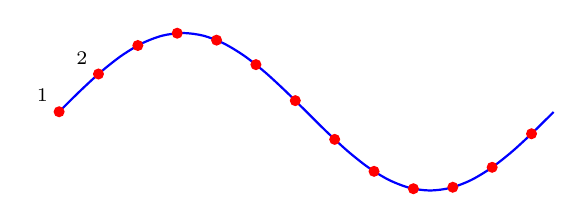
\begin{tikzpicture}[scale=1]
			% Draw a smooth waveform (sine curve as proxy for audio)
			\draw[thick, blue, domain=0:6.28, smooth, variable=\x] 
			plot ({\x}, {sin(\x r)});
			% Mark sample points at regular intervals
			\foreach \x [count=\i] in {0,0.5,...,6.28} {
				\fill[red] (\x, {sin(\x r)}) circle (2pt);
				% Label only the first two samples
				\ifnum\i=1
				\node[above left] at (\x, {sin(\x r)}) {$\feature_1$};
				\fi
				\ifnum\i=2
				\node[above left] at (\x, {sin(\x r)}) {$\feature_2$};
				\fi
			}
		\end{tikzpicture}
		\caption{An audio signal (blue waveform) $\datapoint$ and its discretized signal samples (red dots) which 
			can be used as its \glspl{feature} $\feature_{1},\ldots,\feature_{\nrfeatures}$. \label{fig:audio_features_dict}}
	\end{figure}
	\end{frame}
	
	\begin{frame}{\Gls{featurespace}}
	\begin{itemize} 
		\item often we use a fixed number $\nrfeatures \in \mathbb{N}$ of \glspl{feature} 
		\item stack them into a \gls{featurevec} $\featurevec=\big(\feature_{1},\ldots,\feature_{\nrfeatures}\big)$ 
		\item \glspl{featurevec} belong to some \gls{featurespace} $\featurespace$ 
		\item most widely-used (by far) choice is $\featurespace= \mathbb{R}^{\nrfeatures}$ 
	 \end{itemize} 
	 \vspace*{-4mm}
	 \begin{figure}[H]
	 	\centering
	 	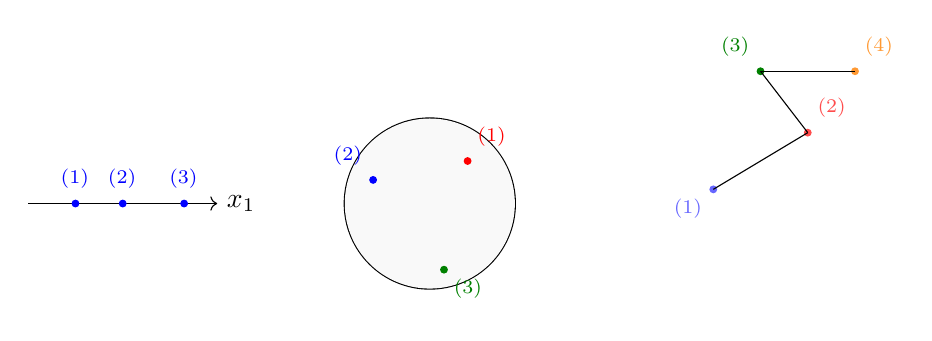
\begin{tikzpicture}[scale=0.6]
	 		% --------- 1D Line Feature Space (left) ---------
	 		\begin{scope}[xshift=0cm]
	 			% Axis
	 			\draw[->] (-0.5, 0) -- (3.5, 0) node[right] {$x_1$};
	 			% Points
	 			\foreach \x/\lbl in {0.5/$\featurevec^{(1)}$, 1.5/$\featurevec^{(2)}$, 2.8/$\featurevec^{(3)}$}
	 			\filldraw[blue] (\x,0) circle (2pt) node[above] {\lbl};
	 			% Label
	 		%	\node at (1.5, -4.0)  {$\featurespace^{(1)}$};
	 		%	\node at (1.5, -6) {(a)};
	 		\end{scope}
	 		% --------- 2-D Bounded (Disk) Feature Space (middle) ---------
	 		\begin{scope}[xshift=8cm]
	 			% Circle boundary
	 			\draw[thick] (0,0) circle (1.8);
	 			\fill[gray!5] (0,0) circle (1.8);
	 			% Points inside circle
	 			\filldraw[red] (0.8, 0.9) circle (2pt) node[anchor=south west] {$\featurevec^{(1)}$};
	 			\filldraw[blue] (-1.2, 0.5) circle (2pt) node[anchor=south east] {$\featurevec^{(2)}$};
	 			\filldraw[green!50!black] (0.3, -1.4) circle (2pt) node[anchor=north west] {$\featurevec^{(3)}$};
	 			% Label
	 		%	\node at (0.5, -4) {$\featurespace^{(2)}$};
	 		%	\node at (0.5, -6) {(b)};
	 		\end{scope}
	 		% --------- Graph-Based Feature Space (right) ---------
	 		\begin{scope}[xshift=14cm, yshift=0.3cm]
	 			% Nodes
	 			\filldraw[blue!60] (0,0) circle (2pt) node[anchor=north east] {$\featurevec^{(1)}$};
	 			\filldraw[red!70] (2,1.2) circle (2pt) node[anchor=south west] {$\featurevec^{(2)}$};
	 			\filldraw[green!50!black] (1,2.5) circle (2pt) node[anchor=south east] {$\featurevec^{(3)}$};
	 			\filldraw[orange!80] (3,2.5) circle (2pt) node[anchor=south west] {$\featurevec^{(4)}$};
	 			% Edges
	 			\draw[-] (0,0) -- (2,1.2);
	 			\draw[-] (2,1.2) -- (1,2.5);
	 			\draw[-] (1,2.5) -- (3,2.5);
	 			% Label
	 	%		\node at (1.5, -4.2) {$\featurespace^{(3)}$};
	 		%	\node at (1.5, -6.2) {(c)};
	 		\end{scope}
	 	\end{tikzpicture}
	 %	\caption{Three different \gls{feature} spaces. (a) A linear space $\featurespace^{(1)} = \mathbb{R}$. (b) A 
	 %		bounded \gls{convex} set $\featurespace^{(2)} \subseteq \mathbb{R}^{2}$. (c) A discrete space 
	 %		$\featurespace^{(3)}$ whose elements are nodes of an undirected \gls{graph}. \label{fig_featurespace_dict}}
	 \end{figure}
	\end{frame}
	
	
		\begin{frame}{\Gls{labelspace}}
\begin{figure}
	\hspace*{-10mm}
	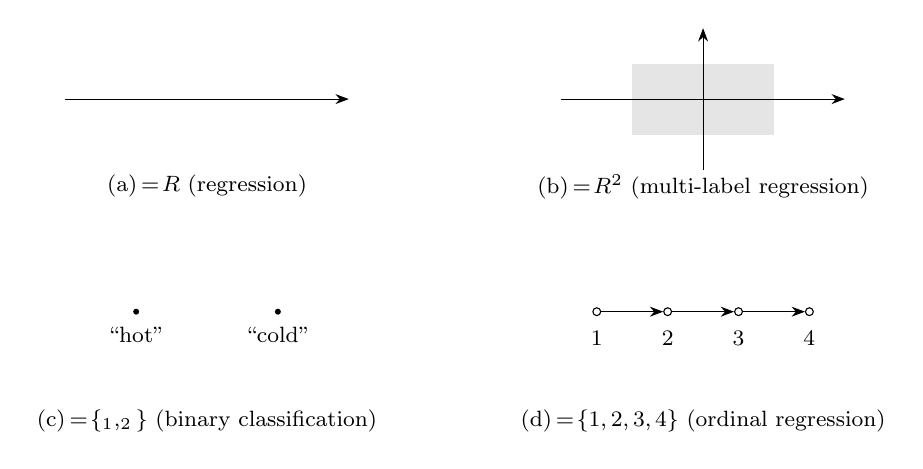
\begin{tikzpicture}[>=Stealth,scale=0.9, font=\footnotesize]
		% (a) Real line for regression
		\begin{scope}[shift={(0,0)}]
			\draw[->] (-2,0) -- (2,0);
			\node[below=6pt] at (0,-0.7) {(a) $\labelspace\!=\!\mathbb{R}$ (\gls{regression})};
		\end{scope}
		% (b) Plane for multi-label regression
		\begin{scope}[shift={(7,0)}]
			% shaded rectangle
			\fill[gray!20] (-1,-0.5) rectangle (1,0.5);
			\draw[->] (-2,0) -- (2,0);
			\draw[->] (0,-1) -- (0,1);
			\node[below=6pt] at (0,-0.7) {(b) $\labelspace\!=\!\mathbb{R}^{2}$ (multi-label \gls{regression})};
		\end{scope}
		% (c) Binary classification
		\begin{scope}[shift={(0,-3)}]
			\fill (-1,0) circle (1.2pt) node[below=2pt] {\text{``hot''}};
			\fill ( 1,0) circle (1.2pt) node[below=2pt] {\text{``cold''}};
			\node[below=14pt] at (0,-0.7) {(c) $\labelspace\!=\!\{\truelabel_{1},\truelabel_{2}\}$ (binary \gls{classification})};
		\end{scope}
		% (d) Ordinal regression: directed chain
		\begin{scope}[shift={(7,-3)}]
			\node[circle, inner sep=1pt, draw] (n1) at (-1.5,0) {};
			\node[circle, inner sep=1pt, draw] (n2) at (-0.5,0) {};
			\node[circle, inner sep=1pt, draw] (n3) at ( 0.5,0) {};
			\node[circle, inner sep=1pt, draw] (n4) at ( 1.5,0) {};
			\draw[->] (n1) -- (n2);
			\draw[->] (n2) -- (n3);
			\draw[->] (n3) -- (n4);
			\node[below=2pt of n1] {1};
			\node[below=2pt of n2] {2};
			\node[below=2pt of n3] {3};
			\node[below=2pt of n4] {4};
			\node[below=14pt] at (0,-0.7) {(d) $\labelspace\!=\!\{1,2,3,4\}$ (ordinal \gls{regression})};
		\end{scope}
	\end{tikzpicture}
	\caption{\label{fig_label_spaces_dict}	Examples of \glspl{labelspace} and corresponding \gls{ml} flavours.}
\end{figure}
	\end{frame}
	
	
	
\begin{frame}{Goal of \gls{ml}: Predict \Gls{label} from \Glspl{feature}}
		% Image as a datapoint
\begin{figure}[htbp]
	\centering
	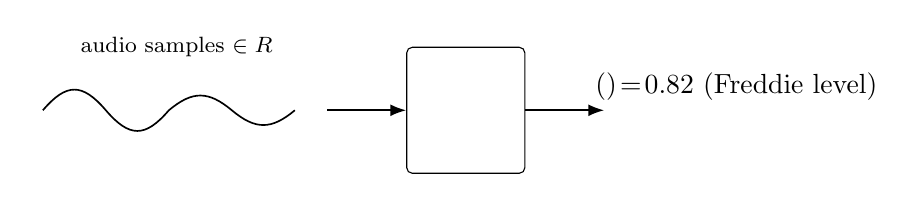
\begin{tikzpicture}[
		>=Latex, node distance=2.0cm,
		box/.style={draw, rounded corners=2pt, inner sep=6pt},
		label/.style={font=\footnotesize},
		thinline/.style={line width=0.6pt}
		]
		% % --- Input: audio signal ---
		\node[minimum width=3.8cm, minimum height=1.6cm] (audio) {};
		%\node[label, above=1mm of audio] {$\mathcal{X}$};
		\node[label] at (audio.north) [yshift=0mm] {audio samples $\featurevec \in \mathbb{R}^{\nrfeatures}$};
		% % A tiny waveform inside the audio box
		\begin{scope}
			%\clip (audio.south west) ++(0.15,0.15) rectangle ($(audio.north east)+(-0.15,-0.15)$);
			\draw[thinline]
			($(audio.west)+(0.2,0)$) .. controls +(.3,.35) and +(-.3,.35) .. ++(0.8,0)
			.. controls +(.3,-.35) and +(-.3,-.35) .. ++(0.8,0)
			.. controls +(.3,.25) and +(-.3,.25) .. ++(0.8,0)
			.. controls +(.3,-.25) and +(-.3,-.25) .. ++(0.8,0);
		\end{scope}
		% % --- Hypothesis map ---
		\node[box,right=1.0cm of audio, minimum width=1.5cm, minimum height=1.6cm] (model)
		{$\hypothesis$};
		\draw[->,thinline] (audio) -- (model) ; %node[midway,above,label] {features \& inference};
		% % --- Output: rating bar ---
		\node[right=1.0cm of model, minimum width=3.2cm, minimum height=1.6cm] (rating) {};
		\node[label, align=center] at ($(rating.north)+(0,-6mm)$)
		{};
		% % Draw a minimalist horizontal score bar
		\coordinate (barL) at ($(rating.west)+(0.4,0)$);
		\coordinate (barR) at ($(rating.east)+(-0.4,0)$);
		\def\score{0.82}
		\coordinate (ptr) at ($(barL)!{\score}!(barR)$);
		%\draw[thinline] (ptr) -- ++(0,-0.28);
		%\fill (ptr) circle (1.2pt);
		\node[yshift=3mm, align= left, xshift=-7mm] at (ptr) {$\hypothesis(\featurevec)\!=\!0.82$ (Freddie level)};
		%\node[label, at ptr, yshift=2mm] {$\hypothesis(\featurevec)\!=\!0.82 (\approx \mbox{Freddie level})$};
		\draw[->,thinline] (model) -- (rating);
	\end{tikzpicture}
	\caption{\label{fig:hypothesis_dict} A \gls{hypothesis} $\hypothesis: \featurespace \rightarrow \labelspace$ maps the \glspl{feature} 
		$\featurevec \in \featurespace$ of a \gls{datapoint} to a \gls{prediction} $\hypothesis(\featurevec) \in \labelspace$ of the \gls{label}. 
		For example, the \gls{ml} application \url{https://freddiemeter.withyoutube.com/} uses the samples of an audio 
		recording as \glspl{feature} predict how closely a person’s singing resembles that of Freddie Mercury.
	}
\end{figure}
	\end{frame}
	
	\begin{frame}{From \Glspl{feature} to \Gls{prediction}}
	\begin{center}
		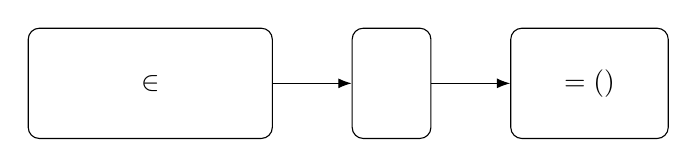
\begin{tikzpicture}[>=Latex, node distance=1.6cm, box/.style={draw, rounded corners, inner sep=6pt}]
			\node[box, minimum width=3.1cm, minimum height=1.4cm] (x) {\(\featurevec \in \featurespace\)};
			\node[box, right=1 cm of x, minimum width=1cm, minimum height=1.4cm] (h) {\(\hypothesis\)};
			\node[box, right=1 cm of h, minimum width=2.0cm, minimum height=1.4cm] (y) {$\predictedlabel=\hypothesis(\featurevec)$};
			\draw[->] (x) -- (h);
			\draw[->] (h) -- (y);
		\end{tikzpicture}
	\end{center}
	
	\small {\bf Core Problem of \gls{ml}} given \gls{data} \(\{(\featurevec^{(\sampleidx)},\truelabel^{(\sampleidx)})\}_{\sampleidx=1}^{\samplesize}\) 
	and \gls{model} \(\hypospace\),
	learn (or find) \(\widehat{\hypothesis}\in\hypospace\) such that $\widehat{\hypothesis}(\featurevec) \approx \truelabel$ for any \gls{datapoint} 
	with \glspl{feature} $\featurevec$ and \gls{label} $\truelabel$.
\end{frame}
	
		\begin{frame}{ \Gls{model} = A Set of \Gls{hypothesis} Maps}
		\begin{figure}[H]
		\centering
		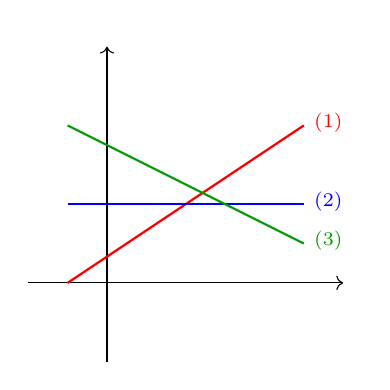
\begin{tikzpicture}[scale=1]
			\draw[->] (-1,0) -- (3,0) node[right] {$\featurespace$};
			\draw[->] (0,-1) -- (0,3) node[above] {$\labelspace$};
			\draw[thick, red] (-0.5,0) -- (2.5,2) node[right] {$\hypothesis^{(1)}$};
			\draw[thick, blue] (-0.5,1) -- (2.5,1) node[right] {$\hypothesis^{(2)}$};
			\draw[thick, green!60!black] (-0.5,2) -- (2.5,0.5) node[right] {$\hypothesis^{(3)}$};
		%	\node at (1.5,-1.2) {(a)};
		\end{tikzpicture}
		\caption{A \gls{hypospace} $\hypospace = \big\{ \hypothesis^{(1)},\hypothesis^{(2)},\hypothesis^{(3)} \big\}$ 
			consisting of three \glspl{linearmap}.  \label{fig_model_dict}}
	\end{figure}
	Which one of the \gls{hypothesis} maps is the best?
	\end{frame}
	
	
\begin{frame}{ \Gls{lossfunc}}
\begin{figure}[H]
	\begin{center}
		\begin{tikzpicture}[scale = 0.7,% enlarge arrowheads globally:
			every axis/.append style={
				axis line style={-Latex, thick},
				tick style={thick}
			}]
			\begin{axis}
				[axis x line=center,
				axis y line=center,
				xlabel={},
				xlabel style={below right},
				ylabel style={above right},
				xtick=\empty,
				ytick=\empty,
				xmin=-5,
				xscale = 1.4, 
				xmax=5,
				ymin=-0.5,
				ymax=2.5,
				clip=false % <-- ensures labels are not cut off
				]
				% Logistic loss: \ell(x) = ln(1 + e^{-x})
				\addplot[red, line width=0.5mm,thick,domain=-2:4] {ln(1 + exp(-x))} node[pos=0.95, above,xshift=13mm] {\gls{logloss} ${\rm log}(1 + {\rm exp}(-\hypothesis(\feature)\truelabel))$};
				% Absolute error: \ell(x) = |x|
				\addplot[blue, line width=0.5mm, dashed, domain=-4:4] {0.5*abs(x)} node[pos=0.8, right,xshift=3mm,yshift=3mm] {\gls{abserr} $ |\truelabel-\hypothesis(\feature)|$};
				% Squared error: \ell(x) = (1/2) x^2
				\addplot[green!50!black, line width=0.5mm, dotted, domain=-3:3] {0.25*x^2} node[pos=1, right,xshift=0mm] {\gls{sqerrloss}$(\truelabel-\hypothesis(\feature))^2$};
				%\addplot [red, thick] {ln(1 + exp(-x))};    
			\end{axis}
			%\node [above,centered,xshift=-5pt] at (1,5) {$\lossfunc{(\featurevec,\truelabel)}{\hypothesis}$};
			\node [below] at (10,1) {$\hypothesis(\featurevec)$};
			\node [right] at (4,6) {$\lossfunc{(\featurevec,\truelabel)}{\hypothesis}$};
		\end{tikzpicture}
	\end{center}
	\vspace*{-1mm}
\end{figure}
	A \gls{lossfunc} $\lossfunc{(\featurevec,\truelabel)}{\hypothesis}$ measures the error (or ``\gls{loss}''), incurred 
	by predicting the \gls{label} $\truelabel$ of a \gls{datapoint} with \gls{featurevec} $\featurevec$. 
\end{frame}


\begin{frame}{Which \Gls{lossfunc} should we use?}
The choice of \gls{lossfunc} influences  \\[2mm]
\begin{itemize} 
	\item \gls{compasp},  \\[4mm]
	\item \gls{statasp} (\gls{robustness}, \gls{generalization}, \ldots), and    \\[4mm]
	\item \gls{interpretability}  \\[3mm]
\end{itemize} 
of the resulting \gls{ml} method. 
\end{frame}
	
\begin{frame}{Reuse \& Citation}
	\small
	This deck is part of the \textbf{Aalto Dictionary of Machine Learning} (open source).\\
	License: \textbf{CC BY 4.0}. Please cite:
	\emph{Jung, A. et.al. (2025). The Aalto Dictionary of Machine Learning}. DOI: 10.5281/zenodo.17273736.
	
	\medskip
	Source and updates: \url{https://github.com/AaltoDictionaryofML/AaltoDictionaryofML.github.io}
\end{frame}




\end{document}
